\chapter{Caminhos Geodésicos}
\label{geomdiff}

\theoremstyle{definition}
\newtheorem{thm}{Definição}
\newtheorem{defCurveParam}[thm]{Definição}
\newtheorem{defCurveReg}[thm]{Definição}
\newtheorem{defSurfParamReg}[thm]{Definição}
\newtheorem{defSurfForm}[thm]{Definição}
\newtheorem{defSurfRotate}[thm]{Definição}
\newtheorem{defSurfParallel}[thm]{Definição}
\newtheorem{defSurfGeodesic}[thm]{Definição}

O objetivo primário do projeto é visualizar curvas e superfícies.
As curvas são visualizadas apenas em espaço 3D.
As superfícies são visualizadas em espaço 3D e em \textit{Geodesic Tracing}.

O estudo da geometria diferencial de curvas e superfícies é
essencial para o \textit{Geodesic Tracing}, e a teoria foi baseada em \cite{GeomDiff:1}.

\section{Curvas}
Há duas principais maneiras de se definir uma curva na geometria analítica:
por equação paramétrica ou equação implícita.
Esse trabalho apenas considera curvas paramétricas.

\begin{defCurveParam}
Uma curva paramétrica $\gamma$ é uma função $\gamma : I \rightarrow \mathbb{R}^n$, onde $I$ é um intervalo real.
\end{defCurveParam}

\begin{defCurveReg}
Numa curva paramétrica $\gamma$, o vetor tangente pode ser facilmente calculado com $\gamma'(t)$.
Uma curva $\gamma$ é regular quando é diferenciável e $\gamma'(t) \neq 0$ para todo $t \in I$.
\end{defCurveReg}

Nesse trabalho, o intervalo é fechado, e $n=3$. Isso significa que todas as
curvas devem ser definidas no espaço 3D. Para desenhar curvas planares,
uma possibilidade é defini-las no plano $xy$, fazendo $z=0$.

As curvas são desenhadas através de vários segmentos.
Dada uma partição de $I$ de $k$ pontos,
pode-se aproximar a curva pelos segmentos de extremidade $\gamma(t_{i})$ e $\gamma(t_{i-1})$ para $i<k$,
onde $t_i$ é o i-ésimo ponto da partição.
Nesse trabalho, a partição depende apenas de $k$ e é uniforme.
Essa escolha foi feita pois essa é a forma mais simples de se implementar.
Porém, dependendo da curvatura de $\gamma$, o intervalo fixo entre os pontos pode
ser demasiadamente pequeno, custando performance, ou demasiadamente grande,
degradando a estética.

\section{Superfícies}
Assim como as curvas, apenas superfícies parametrizadas regulares
serão consideradas nesse trabalho, e apenas definidas em um
espaço ambiente 3D.

\begin{defSurfParamReg}
Uma superfície parametrizada regular $\sigma$ é uma função suave
$\sigma :  I_1 \times I_2 \rightarrow \mathbb{R}^3$,
onde $I_1$ e $I_2$ são intervalos fechados reais.
Além disso, os vetores tangentes $\sigma_u(u,v)$ e $\sigma_v(u,v)$
devem ser linearmente independentes.
\end{defSurfParamReg}

As superfícies são desenhadas através de vários triângulos,
a partir de partições dos intervalos $I_1$ e $I_2$.
Juntas, as partições formam uma grade de retângulos, e cada retângulo pode ser dividido em 2 triângulos.
Esses são os triângulos desenhados.
De forma similar às curvas, essa escolha é a mais simples.
Há maneiras mais inteligentes de escolher as partições, considerando os vetores tangentes,
seus tamanhos e o ângulo formado pelos vetores.

\subsection{Primeira forma fundamental}
\begin{defSurfForm}
Numa superfície parametrizada regular,
a primeira forma fundamental no ponto paramétrico $(u,v)$ é definida como
\[
    \left[
        \begin{array}{cc}
            \sigma_u \cdot \sigma_u & \sigma_u \cdot \sigma_v \\
            \sigma_v \cdot \sigma_u & \sigma_v \cdot \sigma_v
        \end{array}
    \right]
    = 
    \left[
        \begin{array}{cc}
            E & F \\
            F & G
        \end{array}
    \right]
\]
onde as funções são todas aplicadas no ponto $(u,v)$.
\end{defSurfForm}

Os vetores $\sigma_u$ e $\sigma_v$ formam uma base do espaço tangente.
O produto escalar de dois vetores tangentes 
$x = x_1 \sigma_u + x_2 \sigma_v$ e $y = y_1 \sigma_u + y_2 \sigma_v$ pode ser calculado da seguinte forma:
\[x\cdot y = (x_1 \sigma_u + x_2 \sigma_v) \cdot (y_1 \sigma_u + y_2 \sigma_v)\]
\[x\cdot y = x_1 y_1 E + x_1 y_2 F + x_2 y_1 F + x_2 y_2 G\]

O produto depende apenas dos coeficientes e da primeira forma fundamental.
Isso significa que distâncias e ângulos podem ser calculados
sem se referir ao espaço ambiente da parametrização, ou seja, de forma intrínseca.

\subsection{Rotação}
Para a aplicação, é necessário rotacionar vetores no espaço tangente.
É possível rotacionar um vetor apenas usando seus componentes e
a primeira forma fundamental.

Seja $w = u\sigma_u+v\sigma_v$ o vetor a ser rotacionado e $\theta$ o ângulo da rotação.
A base $\{\sigma_u, \sigma_v\}$ do espaço tangente pode ser ortogonalizada.
Com uma base ortogonal, a rotação é feita com a matriz de rotação.

A nova base pode ser escrita como:
\begin{align*}
    \sigma'_u &= \frac{\sigma_u}{E}\\
    \sigma'_v &= \frac{\sigma_v-\frac{F\sigma_u}{E}}{R}\\
    R &= \sqrt{EG-F^2}
\end{align*}

Note que os vetores são ortogonais e de mesmo comprimento.
Apesar do comprimento não ser 1, a matriz de rotação funciona corretamente.

Para achar os componentes de $w$ na nova base, basta observar:
$w = u'\sigma'_u+v'\sigma'_v = u'\frac{\sigma_u}{E} + v'\frac{\sigma_v}{R}-v'\frac{\sigma_uF}{RE}$

Então
\begin{align*}
    u' &= uE + vF\\
    v' &= vR
\end{align*}

\[w' = \left(u'\text{cos}\theta-v'\text{sin}\theta\right)\sigma'_u + \left(u'\text{sin}\theta+v'\text{cos}\theta\right)\sigma'_v\]
\[w' = \left(u\text{cos}\theta-\frac{uF+vG}{R}\text{sin}\theta\right)\sigma_u+\left(\frac{uE+vF}{R}\text{sin}\theta+v\text{cos}\theta\right)\sigma_v\]


\begin{defSurfRotate}
Seja $w = u\sigma_u+v\sigma_v$ um vetor tangente à superfície $\sigma$.
O vetor $w$ rotacionado pelo ângulo $\theta$ é
\[w' = \left(u\text{cos}\theta-\frac{uF+vG}{R}\text{sin}\theta\right)\sigma_u+\left(\frac{uE+vF}{R}\text{sin}\theta+v\text{cos}\theta\right)\sigma_v\]
\end{defSurfRotate}

Como esperado, esse vetor só depende da primeira forma fundamental,
dos componentes originais e do ângulo de rotação.

\subsection{Transporte Paralelo}
\begin{defSurfParallel}
Seja $\gamma$ uma curva sobre a superfície e $v$ um campo vetorial tangente à $\sigma$ definido sobre a curva $\gamma$.
Diz-se que $v$ é paralelo ao longo de $\gamma$ quando $v'$ é ortogonal à superfície $\sigma$
para qualquer ponto de $\gamma$. Ou seja,
\[v'(t) \perp \{\sigma_u(\gamma(t)), \sigma_v(\gamma(t))\}\]
para todo ponto $t \in I$ da curva.
\end{defSurfParallel}

Nesse caso, um ser sobre a superfície não observaria mudanças em $v$ ao traçar a curva $\gamma$.
A variação de $v$ se dá ortogonalmente à superfície, logo não seria percebida pelo ser.
Diz-se que o vetor $v$ está sendo transportado paralelamente ao longo de $\gamma$.

Sejam $v$ e $w$ vetores paralelos ao longo de $\gamma$(transportados paralelamente).
Então o produto escalar $v \cdot w$ é constante, pois $(v \cdot w)' = v' \cdot w + v \cdot w' = 0$.
Como o produto escalar pode definir as noções de comprimento e ângulo, vetores transportados
paralelamente à uma curva mantém seus comprimentos e ângulos entre si.

\subsection{Equação de um caminho geodésico}
\begin{defSurfGeodesic}
Uma curva regular $\gamma$ sobre a superfície é dita geodésica quando
$\gamma'$ é paralelo ao longo de $\gamma$.
\end{defSurfGeodesic}

Nesse caso, um ser perceberia $\gamma'$(velocidade) como constante, e a curva $\gamma$ pode
ser considerada como reta nesse espaço.

Uma curva $\gamma$ é uma curva geodésica quando satisfaz o sistema \ref{geoeq} \cite{GeomDiff:1}.
\begin{equation}
\label{geoeq}
    \left\{\begin{array}{cc}
        \dfrac{1}{2}\left(E_u(u')^2 + 2F_uu'v' + G_u(v')^2\right) & = \dfrac{d}{dt}(Eu' + Fv') \vspace{6pt}\\
        \dfrac{1}{2}\left(E_v(u')^2 + 2F_vu'v' + G_v(v')^2\right) & = \dfrac{d}{dt}(Fu' + Gv')
    \end{array}\right.
\end{equation}

Esse sistema pode ser reescrito como o sistema \ref{geoeq2}.

\begin{equation}
\label{geoeq2}
        2
        \begin{pmatrix}
            E & F \\
            F & G
        \end{pmatrix}
        \begin{pmatrix}
            u'' \\
            v''
        \end{pmatrix}
        =
        \begin{pmatrix}
            v'^2(G_u-2F_v)-u'^2E_u-2u'v'E_v \\
            u'^2(E_v-2F_u)-v'^2G_v-2u'v'G_u
        \end{pmatrix}
\end{equation}

Como a superfície é regular, $u''$ e $v''$ são únicos, pois a primeira forma
fundamental é invertível.

Note que a aceleração $(u'', v'')$ pode ser obtida em função da posição $(u,v)$
e velocidade $(u', v')$: $(u'', v'') = g(u, v, u', v')$.

Esse é um sistema de equações diferenciais ordinárias de primeira ordem.
Sua solução depende de uma posição e uma velocidade inicial.
Na maioria das superfícies interessantes, esse sistema é muito difícil, ou até impossível,
de resolver analiticamente.

\subsection{\textit{Geodesic Tracing}}
O \textit{Geodesic Tracing} gera uma imagem a partir de duas informações:
\begin{itemize}
    \item um ponto $(u,v)$ sobre a superfície, representando a posição da câmera
    \item dois vetores tangentes $X$ e $Y$ no ponto $(u,v)$.
    Os vetores $X$ e $Y$ são de mesmo comprimento($z$), são ortogonais entre si e
    representam a orientação da câmera.
\end{itemize}

A imagem gerada é um quadrado $[-1, +1] \times [-1, +1]$.
O primeiro eixo corresponde ao vetor $X$, e o segundo ao $Y$.

Cada ponto $(x,y)$ é associado a um ponto $(u_1, v_1)$ da superfície.
O ponto $(u_1, v_1)$ é determinado traçando-se uma curva geodésica $\gamma$.
A posição inicial de $\gamma$ é $(u,v)$, e a velocidade inicial é $xX+yY$.
Finalmente, o ponto $(u_1, v_1)$ é definido como $\gamma(1)$.
A distância percorrida, ou comprimento de arco, é o próprio comprimento
da velocidade inicial: $z\sqrt{x^2+y^2}$.

A Figura \ref{img:geotracing} ilustra o \textit{Geodesic Tracing}.
Os vetores em rosa são os vetores $X$ e $Y$, ancorados na câmera, o ponto verde.
O vetor azul é uma combinação linear de $X$ e $Y$, e portanto está no espaço tangente.
O ponto da superfície observado pelo vetor azul é o final da curva vermelha.
A curva é uma geodésica com velocidade inicial igual ao vetor azul, partindo da câmera.

\begin{figure}[!ht]
    \centering
    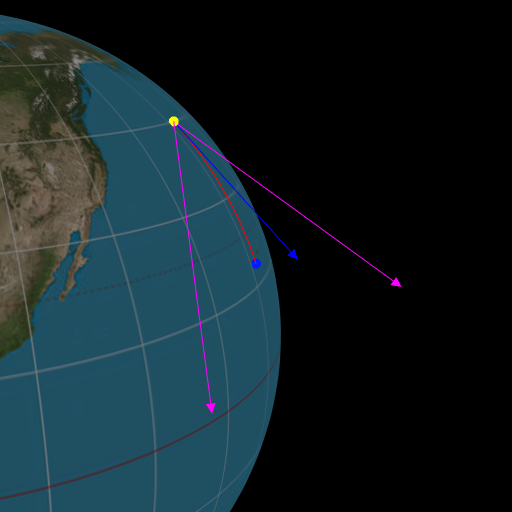
\includegraphics[width=0.6\linewidth]{geotracing.png}
    \caption[Ilustração do \textit{Geodesic Tracing}]{
    Os vetores rosa são os vetores $X$ e $Y$.
    O ponto verde é o centro da câmera. O vetor azul representa um ponto
    da imagem, e corresponde ao ponto vermelho. O ponto é obtido pela curva geodésica
    vermelha, que é determinada pelo vetor azul e pelo ponto verde.}
    \label{img:geotracing}
\end{figure}

A visualização do \textit{Geodesic Tracing} requer uma imagem sobre a superfície.
A cor observada pelo vetor azul, na Figura \ref{img:geotracing}, é a cor da superfície
no ponto vermelho, que é um ponto da imagem original.

\subsection{Interação}
Para compreender melhor o \textit{Geodesic Tracing},
é necessário alterar as condições iniciais e observar as alterações na imagem.

A interação mais simples é a rotação.
Os vetores $X$ e $Y$ são apenas rotacionados por um ângulo $\theta$.
A imagem resultante não se deforma, apenas é rotacionada pelo mesmo ângulo $\theta$.

Outra interação simples é o \textit{zoom}.
Os vetores $X$ e $Y$ são multiplicados por um fator $\alpha > 0$.
Para $\alpha > 1$, a imagem é ampliada, pois as curvas geodésicas são maiores.
Para $\alpha < 1$, a imagem é contraída.

A interação mais interessante é o movimento.
Para se mover na direção $X$, uma geodésica $\gamma$ é traçada na direção $X$.
O novo centro da imagem passa a ser $\gamma(t)$, onde $t$ é o tamanho do passo.
O novo vetor $X$ é a velocidade final($\gamma'(t)$),
que foi transportada paralelamente ao longo
de $\gamma$. O comprimento de $X$ foi preservado.
O novo vetor $Y$ também é transportado paralelamente.
Como visto anteriormente, seu comprimento é preservado e seu ângulo com $X$ também.
Assim, o novo $Y$ é apenas a rotação de $X$ pelo ângulo de $90$ graus.
O comprimento real do passo é $zt$.
De forma similar, a câmera pode se movimentar ao longo de $Y$.

As curvaturas da superfície causam distorções na imagem observada.
Ao se mover, pode-se perceber curvatura pela forma com que a imagem se distorce.
Curvatura gaussiana positiva faz os ``objetos'' expandirem ao se afastar.
Curvatura negativa faz os ``objetos'' contraírem ao se afastar.
Curvatura nula faz os ``objetos'' se moverem de forma rígida.
Além disso, é possível fazer um ``passeio paralelo'': apenas movimentos geodésicos
e sem rotacionar a câmera. Se um passeio paralelo cobre uma área
e retorna à posição inicial, observa-se uma rotação da câmera em relação à direção
inicial. Essa rotação depende da curvatura da superfície na área envolvida.
Uma área de curvatura positiva causa rotações no mesmo sentido do caminho.
O contrário pode ser observado em curvatura negativa, a câmera rotaciona no
sentido oposto ao sentido do caminho: ao andar num círculo em sentido horário,
a câmera é rotacionada do sentido anti-horário.

No caso de um cone, é possível observar uma geometria localmente plana, ou de curvatura nula.
Ao se mover, a imagem se deforma(localmente) rigidamente.
Um passeio paralelo não causa rotações quando a ponta do cone não está no interior do caminho.
Nesse caso, a distância da ponta ao interior da região é completamente irrelevante.
Porém, se a ponta do cone estiver no interior da região percorrida,
observa-se uma rotação de ângulo fixo. Nesse caso, a distância da ponta
ao exterior da região é irrelevante também.

O domínio de parametrização é desprezado no \textit{Geodesic Tracing}.
A fórmula da parametrização é usada no plano $uv$ todo, supondo-se que
a fórmula não faça operações indefinidas, como raiz quadrada de números negativos
ou divisão por zero.
A textura deve ser um arquivo de imagem, sempre retangular.
No quadrado $[0, 1] \times [0, 1]$ se encontra a imagem/textura original.
Se a textura não for quadrada, ela será distorcida. A textura é repetida
para cobrir o plano, simplesmente transladando o quadrado, sem mudar a orientação
da textura.